\documentclass[12pt]{article}
\usepackage{lingmacros}
\usepackage{tree-dvips}
\usepackage{graphicx}
\begin{document}

\section*{Notes for My Paper}

Don't forget to include examples of topicalization.
They look like this:

{\small
\enumsentence{Topicalization from sentential subject:\\
\shortex{7}{a John$_i$ [a & kltukl & [el &
        {\bf l-}oltoir & er & ngii$_i$ & a Mary]]}
{ & {\bf R-}clear & {\sc comp} &
{\bf IR}.{\sc 3s}-love   & P & him & }
{John, (it's) clear that Mary loves (him).}}
}

\subsection*{How to handle topicalization}

I'll just assume a tree structure like (\ex{1}).

{\small
\enumsentence{Structure of A$'$ Projections:\\ [2ex]
\begin{tabular}[t]{cccc}
                  & \node{i}{CP}                                      \\ [2ex]
  \node{ii}{Spec} &              & \node{iii}{C$'$}                   \\ [2ex]
                  & \node{iv}{C} &                  & \node{v}{SAgrP}
\end{tabular}
\nodeconnect{i}{ii}
\nodeconnect{i}{iii}
\nodeconnect{iii}{iv}
\nodeconnect{iii}{v}
}
}

\subsection*{Mood}

Mood changes when there is a topic, as well as when
there is WH-movement.  \emph{Irrealis} is the mood when
there is a non-subject topic or WH-phrase in Comp.
\emph{Realis} is the mood when there is a subject topic
or WH-phrase.

\begin{figure}
  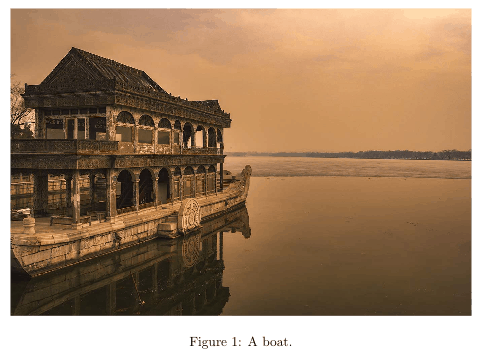
\includegraphics[width=\linewidth]{boat.png}
\end{figure}

\begin{figure}
  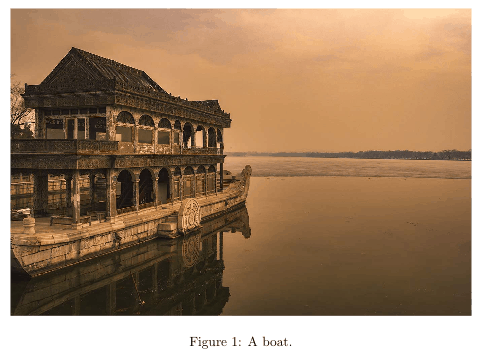
\includegraphics[width=\linewidth]{boat.png}
  \caption{A boat.}
  \label{fig:boat1}
\end{figure}

\end{document}